\documentclass[12pt,letterpaper]{article}
\usepackage{graphicx,textcomp}
\usepackage{natbib}
\usepackage{setspace}
\usepackage{fullpage}
\usepackage{color}
\usepackage[reqno]{amsmath}
\usepackage{amsthm}
\usepackage{fancyvrb}
\usepackage{amssymb,enumerate}
\usepackage[all]{xy}
\usepackage{endnotes}
\usepackage{lscape}
\newtheorem{com}{Comment}
\usepackage{float}
\usepackage{hyperref}
\newtheorem{lem} {Lemma}
\newtheorem{prop}{Proposition}
\newtheorem{thm}{Theorem}
\newtheorem{defn}{Definition}
\newtheorem{cor}{Corollary}
\newtheorem{obs}{Observation}
\usepackage[compact]{titlesec}
\usepackage{dcolumn}
\usepackage{tikz}
\usetikzlibrary{arrows}
\usepackage{multirow}
\usepackage{xcolor}
\newcolumntype{.}{D{.}{.}{-1}}
\newcolumntype{d}[1]{D{.}{.}{#1}}
\definecolor{light-gray}{gray}{0.65}
\usepackage{url}
\usepackage{listings}
\usepackage{color}

\definecolor{codegreen}{rgb}{0,0.6,0}
\definecolor{codegray}{rgb}{0.5,0.5,0.5}
\definecolor{codepurple}{rgb}{0.58,0,0.82}
\definecolor{backcolour}{rgb}{0.95,0.95,0.92}

\lstdefinestyle{mystyle}{
	backgroundcolor=\color{backcolour},   
	commentstyle=\color{codegreen},
	keywordstyle=\color{magenta},
	numberstyle=\tiny\color{codegray},
	stringstyle=\color{codepurple},
	basicstyle=\footnotesize,
	breakatwhitespace=false,         
	breaklines=true,                 
	captionpos=b,                    
	keepspaces=true,                 
	numbers=left,                    
	numbersep=5pt,                  
	showspaces=false,                
	showstringspaces=false,
	showtabs=false,                  
	tabsize=2
}
\lstset{style=mystyle}
\newcommand{\Sref}[1]{Section~\ref{#1}}
\newtheorem{hyp}{Hypothesis}

\title{Problem Set 3}
\date{Applied Stats/Quant Methods 1}
\author{Linette Lim}


\begin{document}
	\maketitle
	\section*{Instructions}
	\begin{itemize}
		\item Please show your work! You may lose points by simply writing in the answer. If the problem requires you to execute commands in \texttt{R}, please include the code you used to get your answers. Please also include the \texttt{.R} file that contains your code. If you are not sure if work needs to be shown for a particular problem, please ask.
	\item Your homework should be submitted electronically on GitHub.
	\item This problem set is due before 23:59 on Sunday November 20, 2022. No late assignments will be accepted.
	\item Total available points for this homework is 80.
	\end{itemize}

		\vspace{.25cm}
	
\noindent In this problem set, you will run several regressions and create an add variable plot (see the lecture slides) in \texttt{R} using the \texttt{incumbents\_subset.csv} dataset. Include all of your code.

	\vspace{.5cm}
\section*{Question 1}
\vspace{.25cm}
\noindent We are interested in knowing how the difference in campaign spending between incumbent and challenger affects the incumbent's vote share. 
	\begin{enumerate}
		\item Run a regression where the outcome variable is \texttt{voteshare} and the explanatory variable is \texttt{difflog}.	\vspace{5cm}
\noindent First, we make sure the global environment is clear and tidyverse is loaded. Then, we enter the data.\\
\lstinputlisting[language=R, firstline=6, lastline=6]{PS3_answers_LinetteLim.R}  
\vspace{.5cm}   
\noindent Then, we use the lm() function to fit a regression model where the outcome variable is voteshare and the explanatory variable is difflog.\\
\vspace{.5cm}
\lstinputlisting[language=R, firstline=10, lastline=12]{PS3_answers_LinetteLim.R}  
\vspace{.5cm}    
\noindent We get:\\
\begin{verbatim}
> summary(diffvote.lm)

Call:
lm(formula = voteshare ~ difflog, data = data)

Residuals:
     Min       1Q   Median       3Q      Max 
-0.26832 -0.05345 -0.00377  0.04780  0.32749 

Coefficients:
            Estimate Std. Error t value Pr(>|t|)    
(Intercept) 0.579031   0.002251  257.19   <2e-16 ***
difflog     0.041666   0.000968   43.04   <2e-16 ***
---
Signif. codes:  0 ‘***’ 0.001 ‘**’ 0.01 ‘*’ 0.05 ‘.’ 0.1 ‘ ’ 1

Residual standard error: 0.07867 on 3191 degrees of freedom
Multiple R-squared:  0.3673,	Adjusted R-squared:  0.3671 
F-statistic:  1853 on 1 and 3191 DF,  p-value: < 2.2e-16
\end{verbatim}
		\item Make a scatterplot of the two variables and add the regression line. 	\vspace{7cm}
\noindent We use the plot() function to make a scatterplot and abline () to add the regression line.\\
\vspace{.5cm}
\lstinputlisting[language=R, firstline=15, lastline=19]{PS3_answers_LinetteLim.R}  
\vspace{.5cm}   
\noindent We get:\\
\begin{figure}[h!]\centering
	\caption{\footnotesize Impact of Difference in Campaign Spend on Incumbent Party Voteshare.}
	\label{fig:plot_1}
	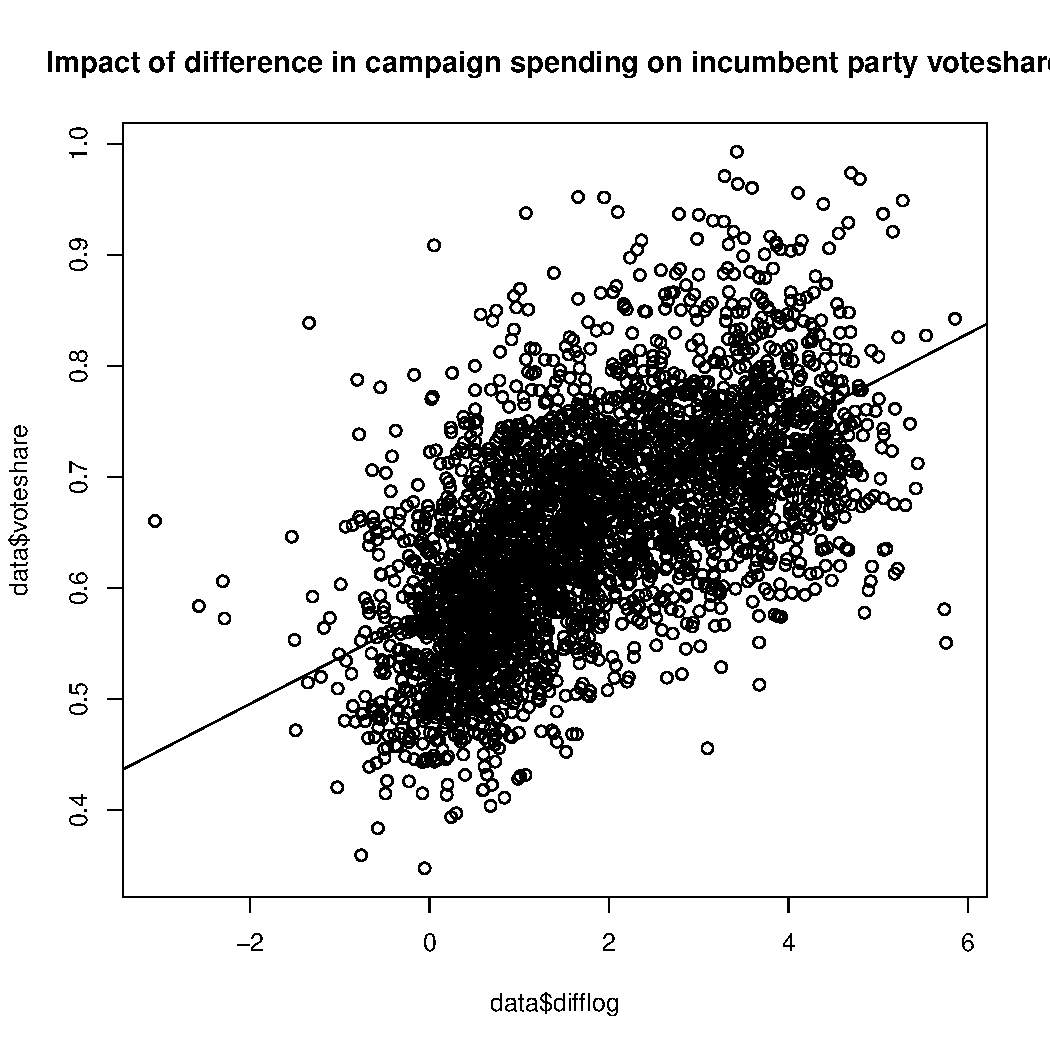
\includegraphics[width=.5\textwidth]{plot1_difflog_voteshare.pdf}
\end{figure}
		\item Save the residuals of the model in a separate object.	\vspace{7cm}
\noindent We use the resid() function to calculate the residuals and then save as separate object.\\
\vspace{.5cm}
\lstinputlisting[language=R, firstline=22, lastline=22]{PS3_answers_LinetteLim.R}  
\vspace{.5cm}   
\noindent Let us plot the residuals using the predict() and segments() functions to check that the assumptions of the model have been satisfied.\\
\vspace{.5cm}
\lstinputlisting[language=R, firstline=24, lastline=25]{PS3_answers_LinetteLim.R}  
\vspace{.5cm}   
\begin{figure}[h!]\centering
	\caption{\footnotesize Residuals and regression line of Plot 1.}
	\label{fig:plot_2}
	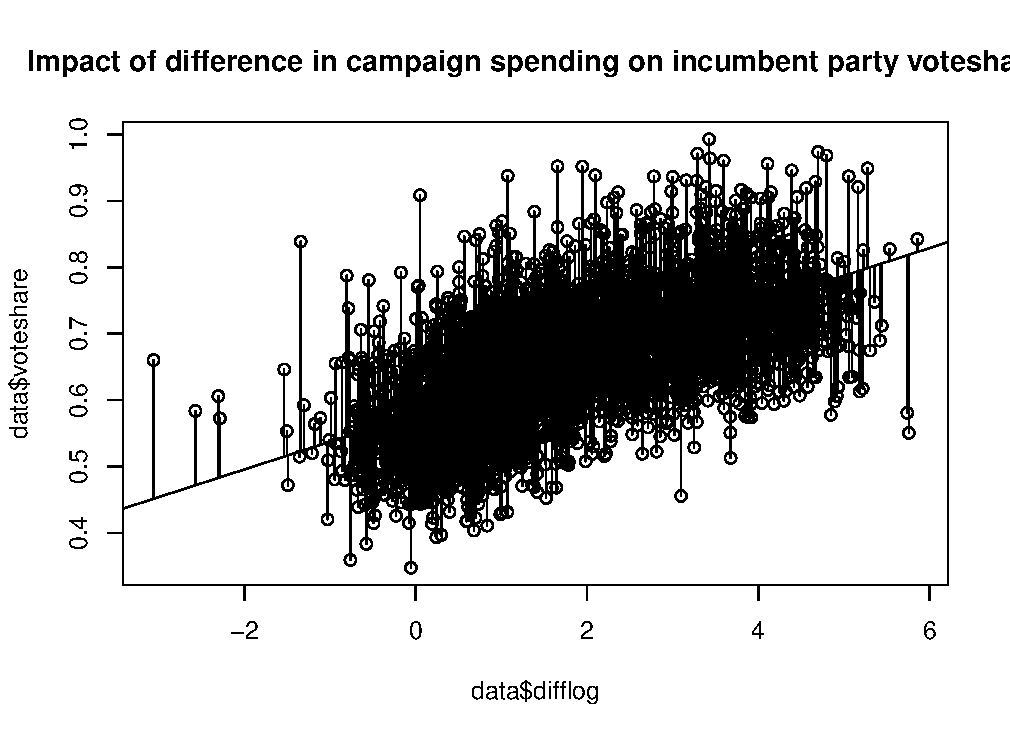
\includegraphics[width=.5\textwidth]{plot2_residuals and regression line.pdf}
\end{figure}
\noindent We want to check that the residuals are zero in expectation (Figure 3).\\
\vspace{.5cm}
\lstinputlisting[language=R, firstline=27, lastline=33]{PS3_answers_LinetteLim.R}  
\vspace{.5cm}  
\begin{figure}[h!]\centering
	\caption{\footnotesize Density of residuals.}
	\label{fig:plot_3}
	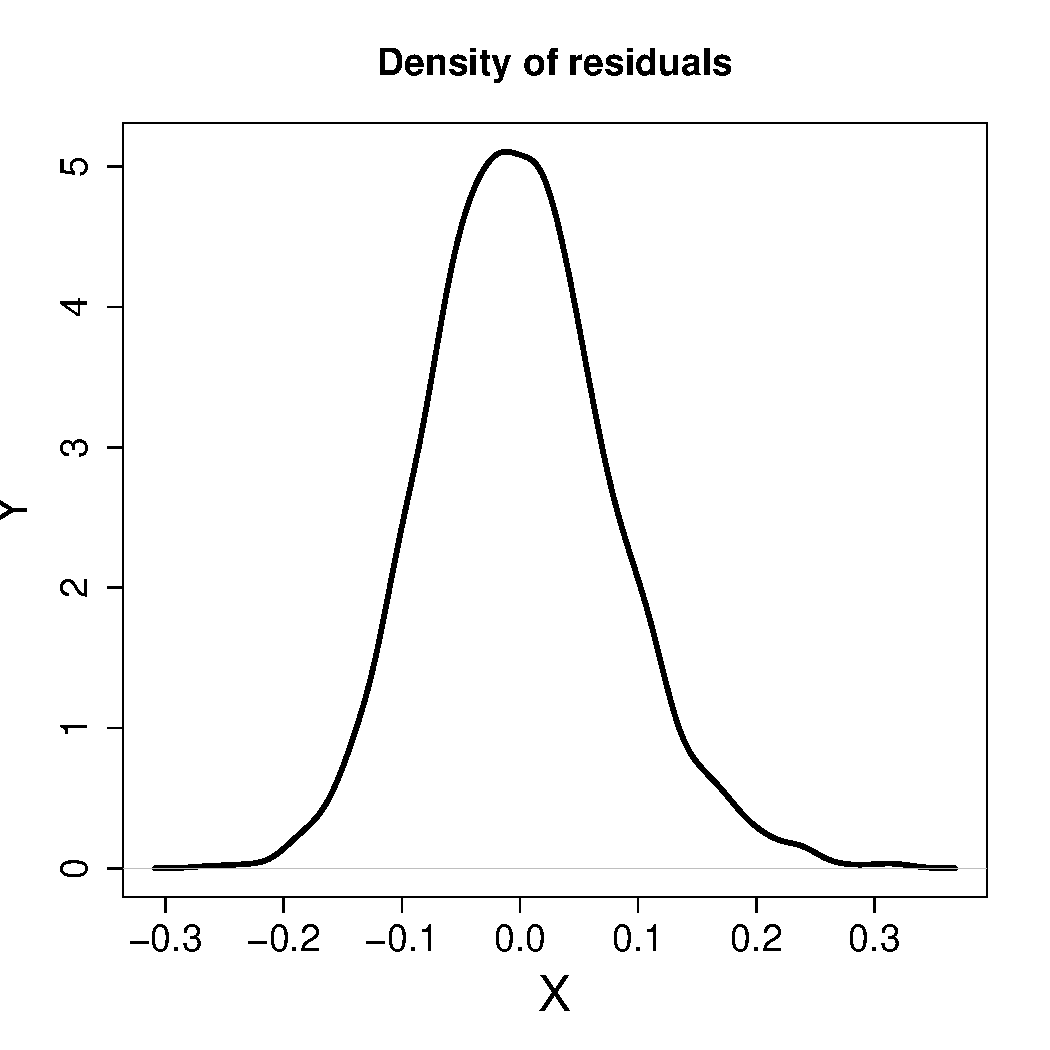
\includegraphics[width=.5\textwidth]{plot3_density of residuals.pdf}
\end{figure}
\noindent We would also expect the residuals to be randomly scattered without showing any  systematic patterns when plotted against the predictor variable (Figure 4):\\
\vspace{.5cm}
\lstinputlisting[language=R, firstline=36, lastline=39]{PS3_answers_LinetteLim.R}  
\vspace{.5cm}  
\begin{figure}[h!]\centering
	\caption{\footnotesize Residual against predictor plot.}
	\label{fig:plot_4}
	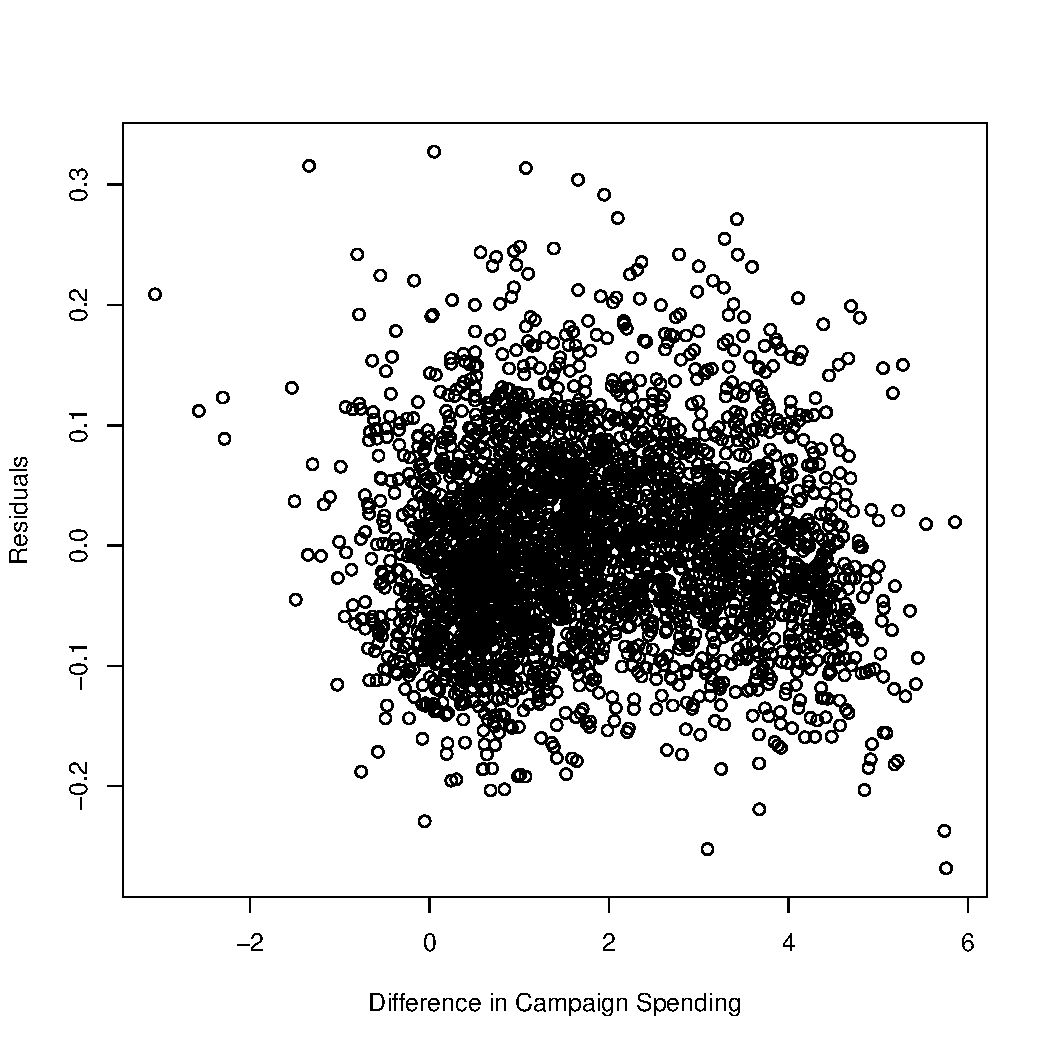
\includegraphics[width=.5\textwidth]{plot4_residual against predictor.pdf}
\end{figure}
		\item Write the prediction equation.
\noindent Using Y = b0 + b1X1 and extracting the coefficients from diffvote.lm in Q1.1, we have: Incumbent party voteshare = 0.58 + 0.04*Difference in Campaign Spending, or Y = 0.58 + 0.04X1\\
	\end{enumerate}
	
\newpage

\section*{Question 2}
\noindent We are interested in knowing how the difference between incumbent and challenger's spending and the vote share of the presidential candidate of the incumbent's party are related.\\
	\begin{enumerate}
		\item Run a regression where the outcome variable is \texttt{presvote} and the explanatory variable is \texttt{difflog}.	\\
\noindent We use lm() to fit a regression model where the outcome variable is presvote and the explanatory variable is difflog.\\
\vspace{.5cm}
\lstinputlisting[language=R, firstline=47, lastline=49]{PS3_answers_LinetteLim.R}  
\vspace{.5cm}  
\noindent We get:\\
\begin{verbatim}
> summary(diffpres.lm)

Call:
lm(formula = presvote ~ difflog, data = data)

Residuals:
     Min       1Q   Median       3Q      Max 
-0.32196 -0.07407 -0.00102  0.07151  0.42743 

Coefficients:
            Estimate Std. Error t value Pr(>|t|)    
(Intercept) 0.507583   0.003161  160.60   <2e-16 ***
difflog     0.023837   0.001359   17.54   <2e-16 ***
---
Signif. codes:  0 ‘***’ 0.001 ‘**’ 0.01 ‘*’ 0.05 ‘.’ 0.1 ‘ ’ 1

Residual standard error: 0.1104 on 3191 degrees of freedom
Multiple R-squared:  0.08795,	Adjusted R-squared:  0.08767 
F-statistic: 307.7 on 1 and 3191 DF,  p-value: < 2.2e-16
\end{verbatim}
		\item Make a scatterplot of the two variables and add the regression line.\\
\noindent We use the plot() to make a scatterplot and abline () to add the regression line. (Figure 5)\\
\lstinputlisting[language=R, firstline=52, lastline=56]{PS3_answers_LinetteLim.R}  
\vspace{.5cm}   
\begin{figure}[h!]\centering
	\caption{\footnotesize Impact of Difference in Campaign Spend on Incumbent Party's Presidential Voteshare.}
	\label{fig:plot_5}
	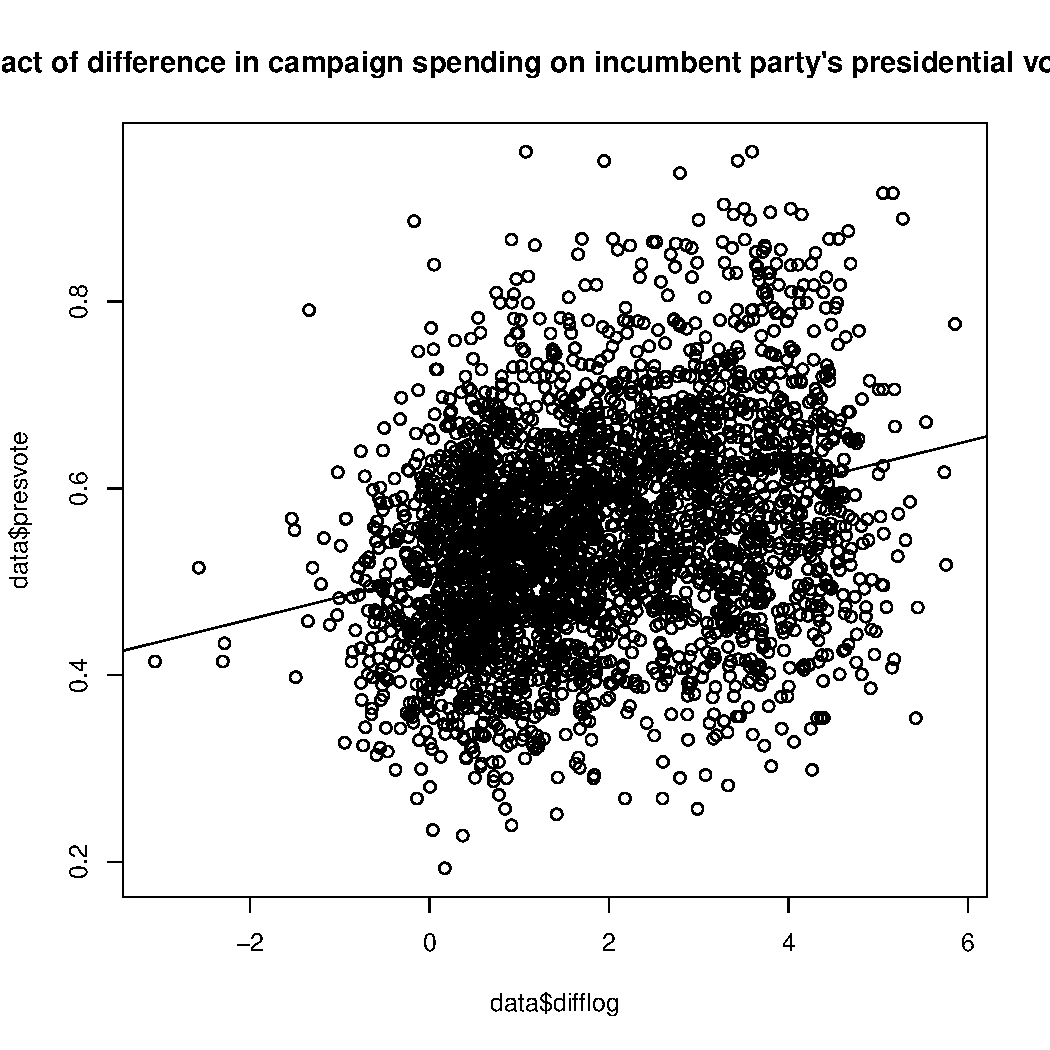
\includegraphics[width=.5\textwidth]{plot5_difflog_presvote.pdf}
\end{figure}
\newpage	
		\item Save the residuals of the model in a separate object.\\
\noindent We use the resid() function to calculate the residuals and then save as separate object.\\
\vspace{.5cm}
\lstinputlisting[language=R, firstline=59, lastline=59]{PS3_answers_LinetteLim.R}  
\vspace{.5cm}   
\noindent Let us plot the residuals using the predict() and segments() functions to check that the assumptions of the model have been satisfied (Figure 6).\\
\vspace{.5cm}
\lstinputlisting[language=R, firstline=61, lastline=62]{PS3_answers_LinetteLim.R}  
\vspace{.5cm}   
\begin{figure}[h!]\centering
	\caption{\footnotesize Residuals and regression line of Plot 5.}
	\label{fig:plot_6}
	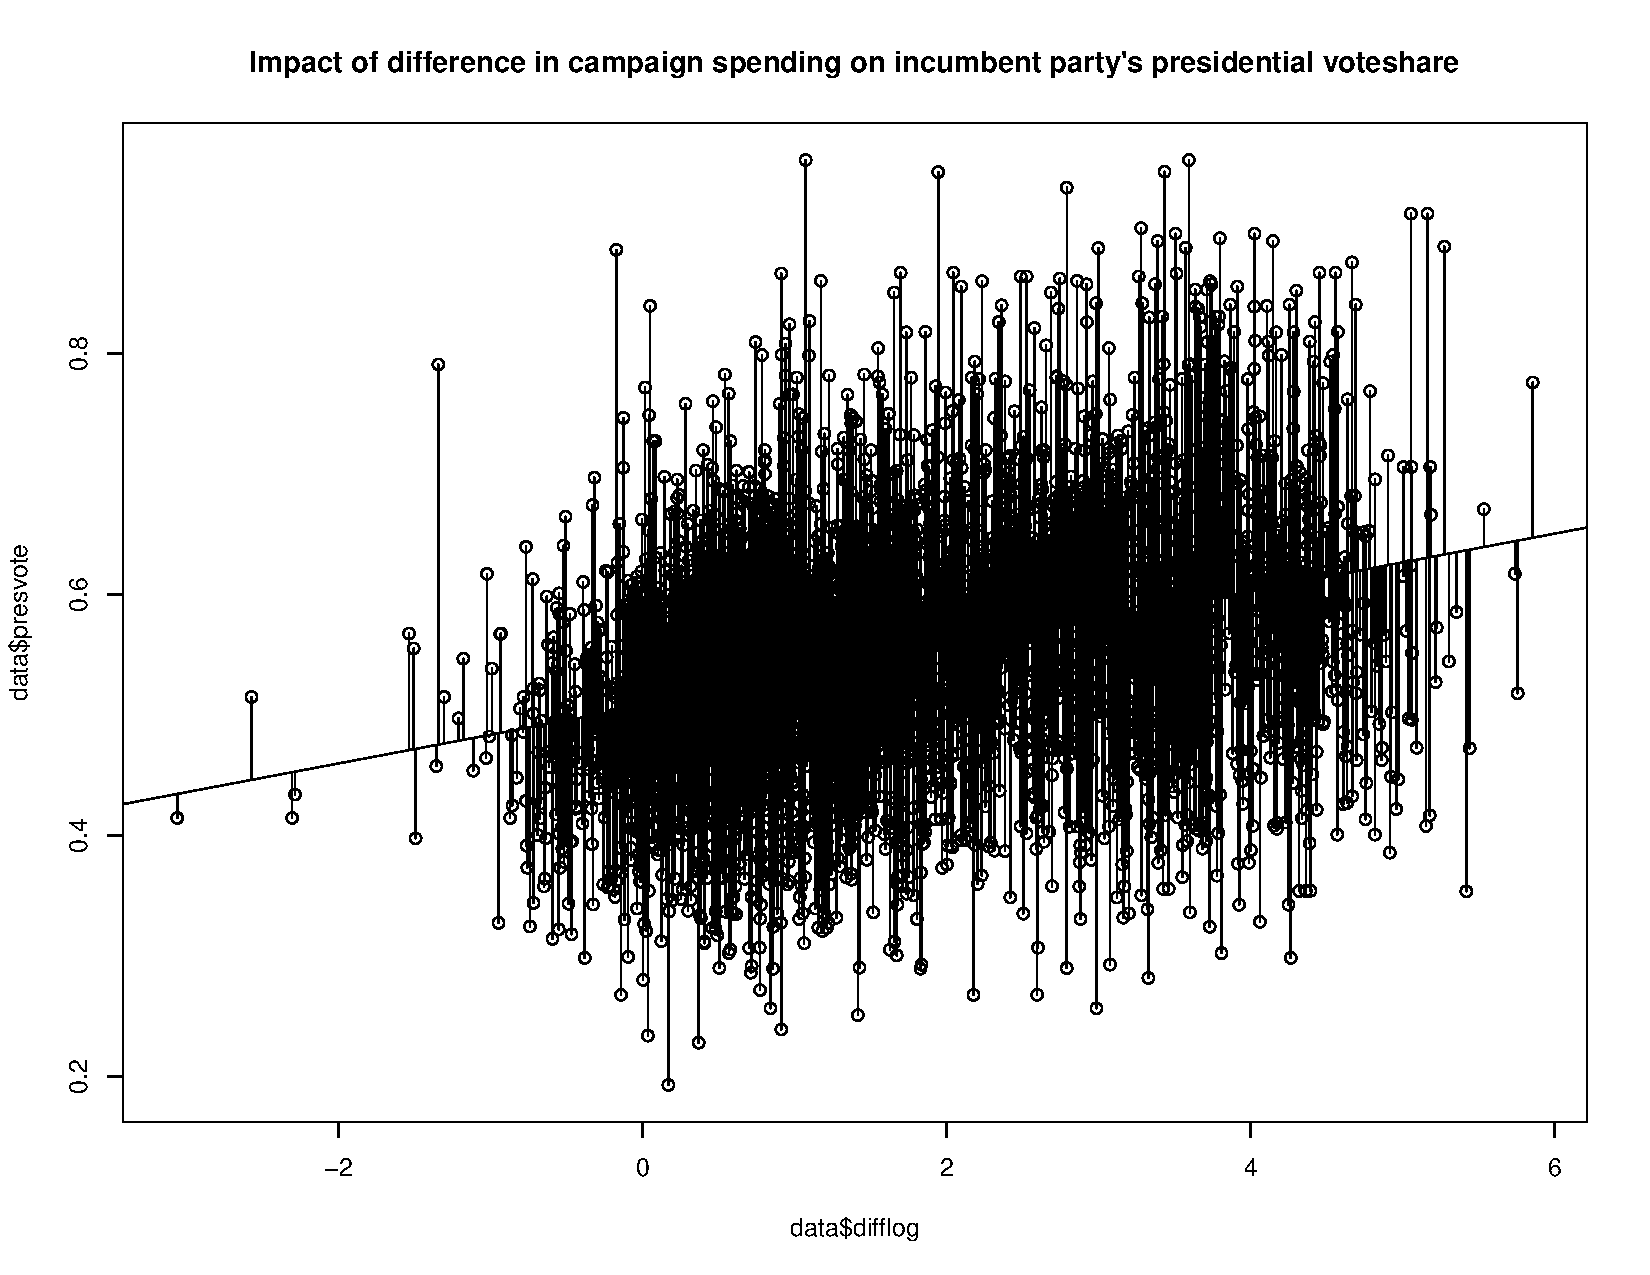
\includegraphics[width=.5\textwidth]{plot6_residuals and regression line.pdf}
\end{figure}
\noindent We want to check that the residuals are zero in expectation (Figure 7).\\
\vspace{.5cm}
\lstinputlisting[language=R, firstline=63, lastline=69]{PS3_answers_LinetteLim.R}  
\vspace{.5cm}  
\begin{figure}[h!]\centering
	\caption{\footnotesize Density of residuals.}
	\label{fig:plot_7}
	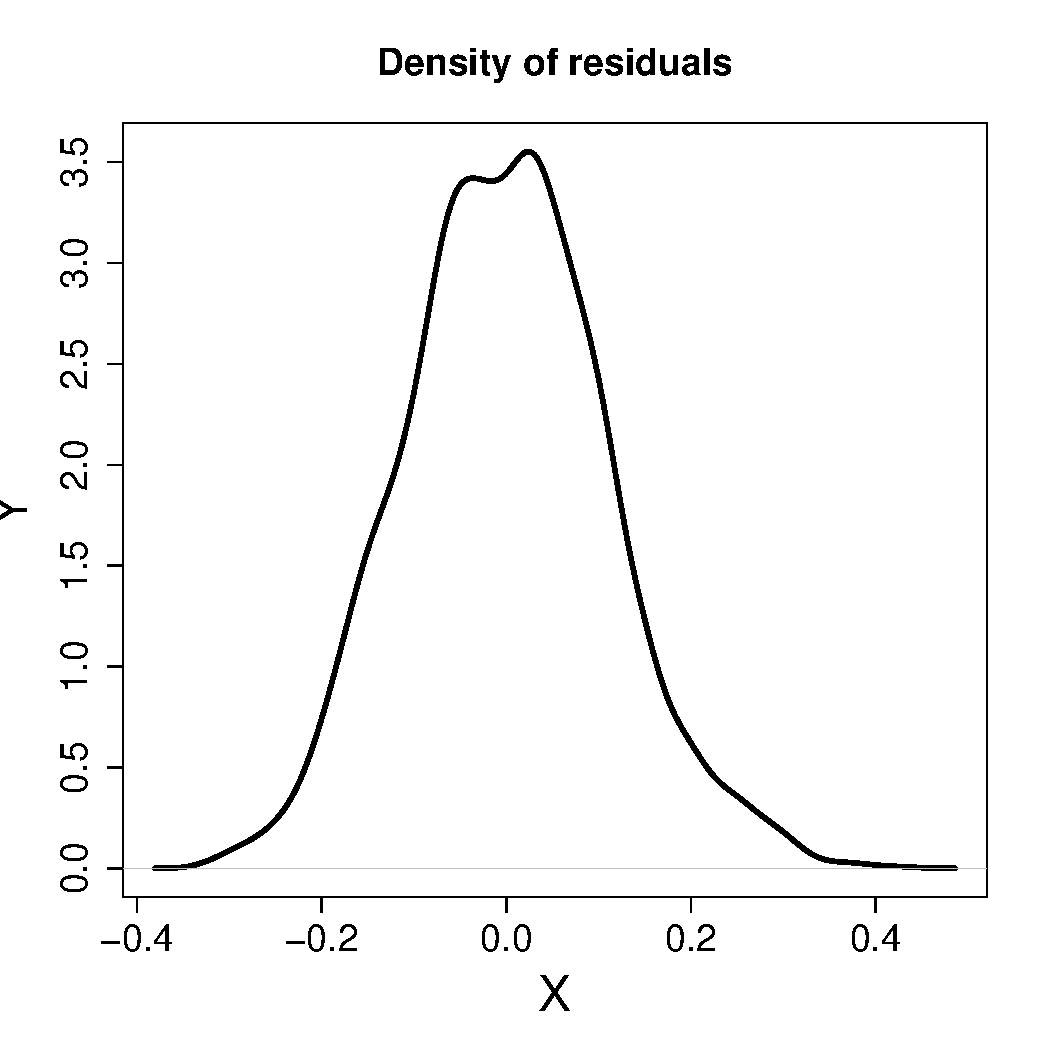
\includegraphics[width=.5\textwidth]{plot7_density of residuals.pdf}
\end{figure}
\newpage	
\noindent We would also expect the residuals to be randomly scattered without showing any  systematic patterns when plotted against the predictor variable (Figure 8):\\
\vspace{.5cm}
\lstinputlisting[language=R, firstline=73, lastline=76]{PS3_answers_LinetteLim.R}  
\vspace{.5cm}  
\begin{figure}[h!]\centering
	\caption{\footnotesize Residual against predictor plot.}
	\label{fig:plot_8}
	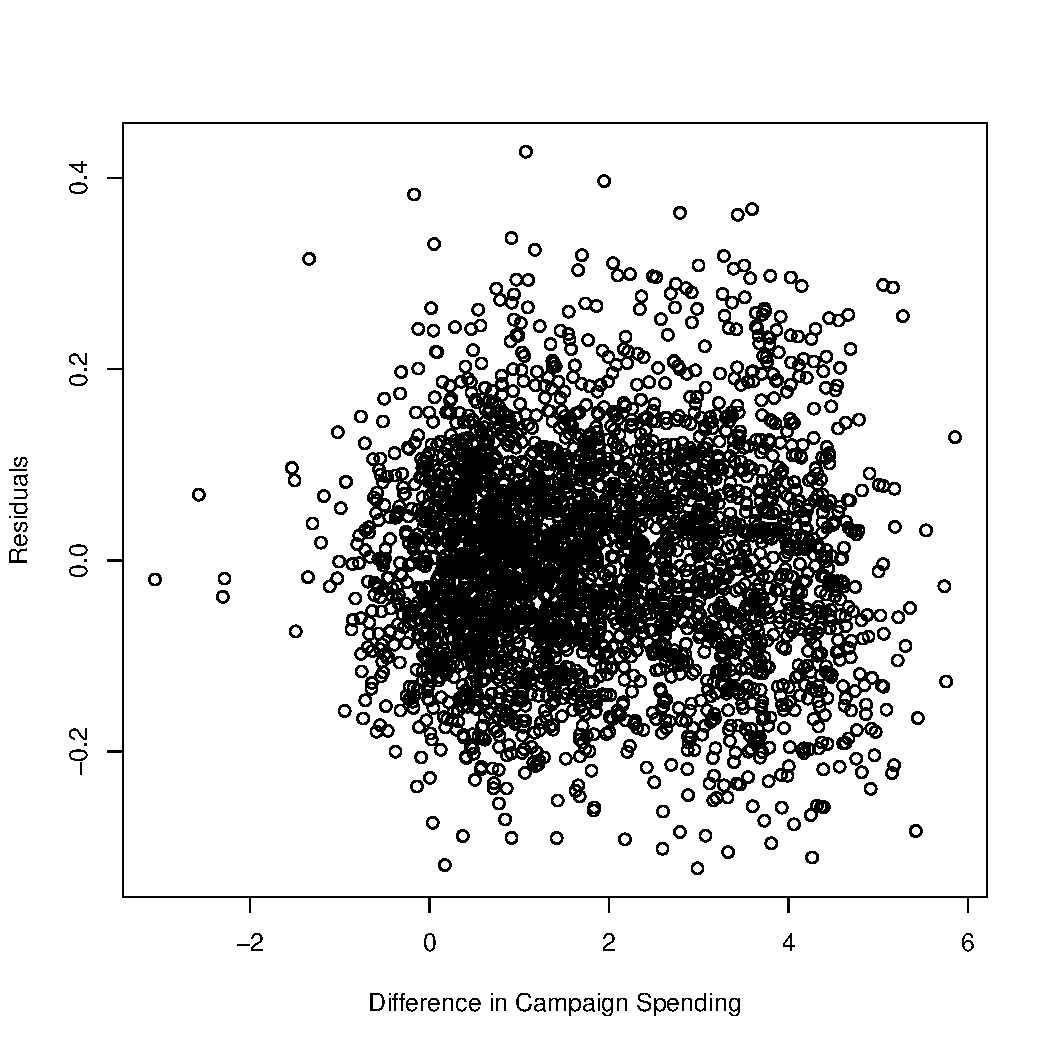
\includegraphics[width=.5\textwidth]{plot8_residual against predictor.pdf}
\end{figure}
		\item Write the prediction equation.
\noindent Using Y = b0 + b1X1 and extracting the coefficients from diffpres.lm in Q2.1, we have: Incumbent party's presidential voteshare = 0.51 + 0.02*Difference in Campaign Spending, or Y = 0.51 + 0.02X1\\
	\end{enumerate}
	
	\newpage	
\section*{Question 3}

\noindent We are interested in knowing how the vote share of the presidential candidate of the incumbent's party is associated with the incumbent's electoral success.\\
	\vspace{.25cm}
	\begin{enumerate}
		\item Run a regression where the outcome variable is \texttt{voteshare} and the explanatory variable is \texttt{presvote}.\\
\noindent We use lm() to fit a regression model where the outcome variable is voteshare and the explanatory variable is presvote.\\
\vspace{.5cm}
\lstinputlisting[language=R, firstline=84, lastline=86]{PS3_answers_LinetteLim.R}  
\vspace{.5cm}  
\noindent We get:\\
\begin{verbatim}
> summary(presvoteshare.lm)

Call:
lm(formula = voteshare ~ presvote, data = data)

Residuals:
     Min       1Q   Median       3Q      Max 
-0.27330 -0.05888  0.00394  0.06148  0.41365 

Coefficients:
            Estimate Std. Error t value Pr(>|t|)    
(Intercept) 0.441330   0.007599   58.08   <2e-16 ***
presvote    0.388018   0.013493   28.76   <2e-16 ***
---
Signif. codes:  0 ‘***’ 0.001 ‘**’ 0.01 ‘*’ 0.05 ‘.’ 0.1 ‘ ’ 1

Residual standard error: 0.08815 on 3191 degrees of freedom
Multiple R-squared:  0.2058,	Adjusted R-squared:  0.2056 
F-statistic:   827 on 1 and 3191 DF,  p-value: < 2.2e-16
\end{verbatim}
			\vspace{5cm}
		\item Make a scatterplot of the two variables and add the regression line. 
\lstinputlisting[language=R, firstline=89, lastline=93]{PS3_answers_LinetteLim.R}  
\vspace{.5cm}  
\begin{figure}[h!]\centering
	\caption{\footnotesize Impact of presvote on voteshare.}
	\label{fig:plot_9}
	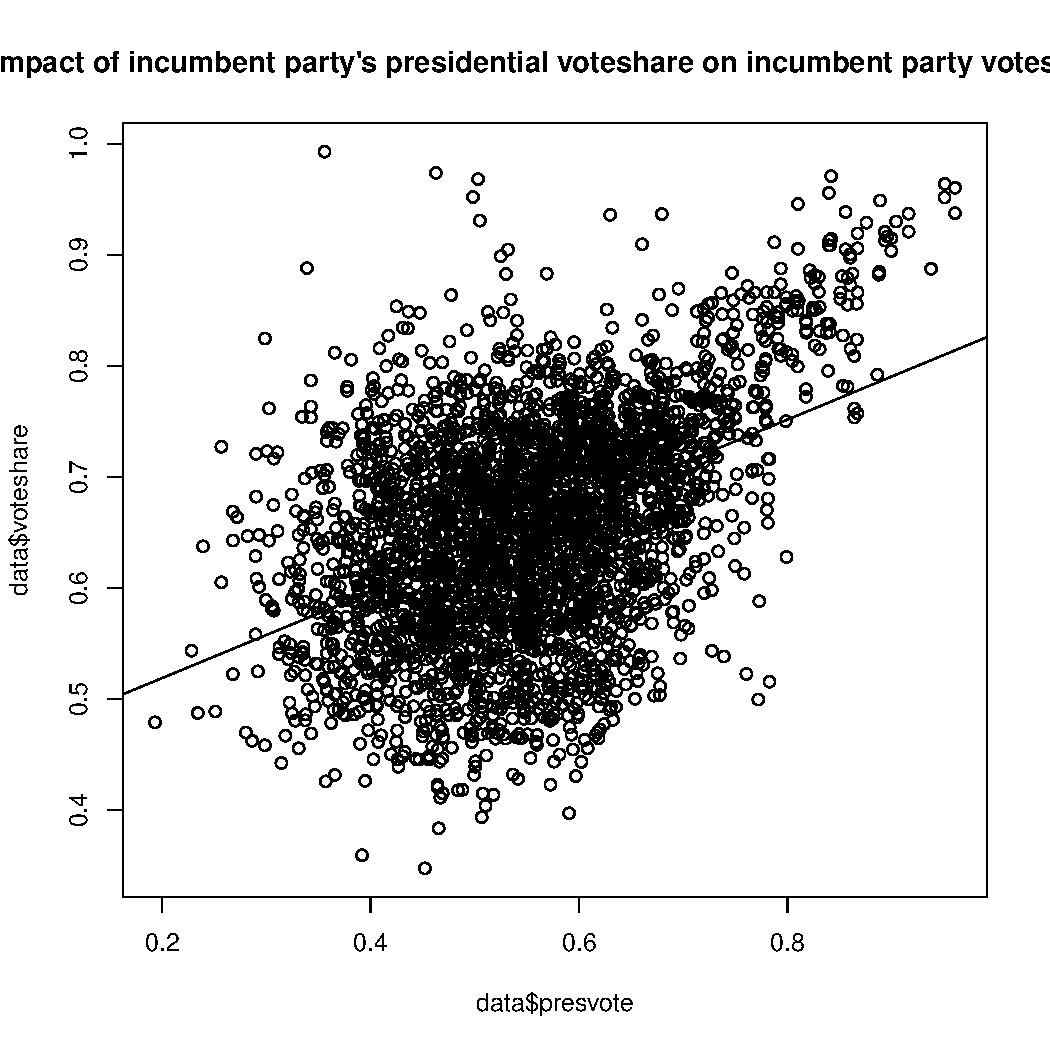
\includegraphics[width=.5\textwidth]{plot9_presvote_voteshare.pdf}
\end{figure}
		\item Write the prediction equation.
\noindent Using Y = b0 + b1X1 and extracting the coefficients from presvoteshare.lm in Q3.1, we have: Incumbent party voteshare = 0.44 + 0.39*incumbent party's presidential voteshare, or Y = 0.44 + 0.39X\\
	\end{enumerate}

\newpage	
\section*{Question 4}
\noindent The residuals from part (a) tell us how much of the variation in \texttt{voteshare} is $not$ explained by the difference in spending between incumbent and challenger. The residuals in part (b) tell us how much of the variation in \texttt{presvote} is $not$ explained by the difference in spending between incumbent and challenger in the district.\\
	\begin{enumerate}
		\item Run a regression where the outcome variable is the residuals from Question 1 and the explanatory variable is the residuals from Question 2.\\
\vspace{.5cm}
\lstinputlisting[language=R, firstline=102, lastline=104]{PS3_answers_LinetteLim.R}  
\vspace{.5cm}  
\noindent We get:\\
\begin{verbatim}
> summary(residuals.lm)

Call:
lm(formula = diffvote.res ~ diffpres.res, data = data)

Residuals:
     Min       1Q   Median       3Q      Max 
-0.25928 -0.04737 -0.00121  0.04618  0.33126 

Coefficients:
               Estimate Std. Error t value Pr(>|t|)    
(Intercept)  -4.860e-18  1.299e-03    0.00        1    
diffpres.res  2.569e-01  1.176e-02   21.84   <2e-16 ***
---
Signif. codes:  0 ‘***’ 0.001 ‘**’ 0.01 ‘*’ 0.05 ‘.’ 0.1 ‘ ’ 1

Residual standard error: 0.07338 on 3191 degrees of freedom
Multiple R-squared:   0.13,	Adjusted R-squared:  0.1298 
F-statistic:   477 on 1 and 3191 DF,  p-value: < 2.2e-16
\end{verbatim}
		\item Make a scatterplot of the two residuals and add the regression line. 	
\noindent We use plot() and abline () to make a scatterplot and add the regression line.\\
\vspace{5cm}
\lstinputlisting[language=R, firstline=107, lastline=111]{PS3_answers_LinetteLim.R}  
\vspace{.5cm}  
\begin{figure}[h!]\centering
	\caption{\footnotesize Residuals plot.}
	\label{fig:plot_10}
	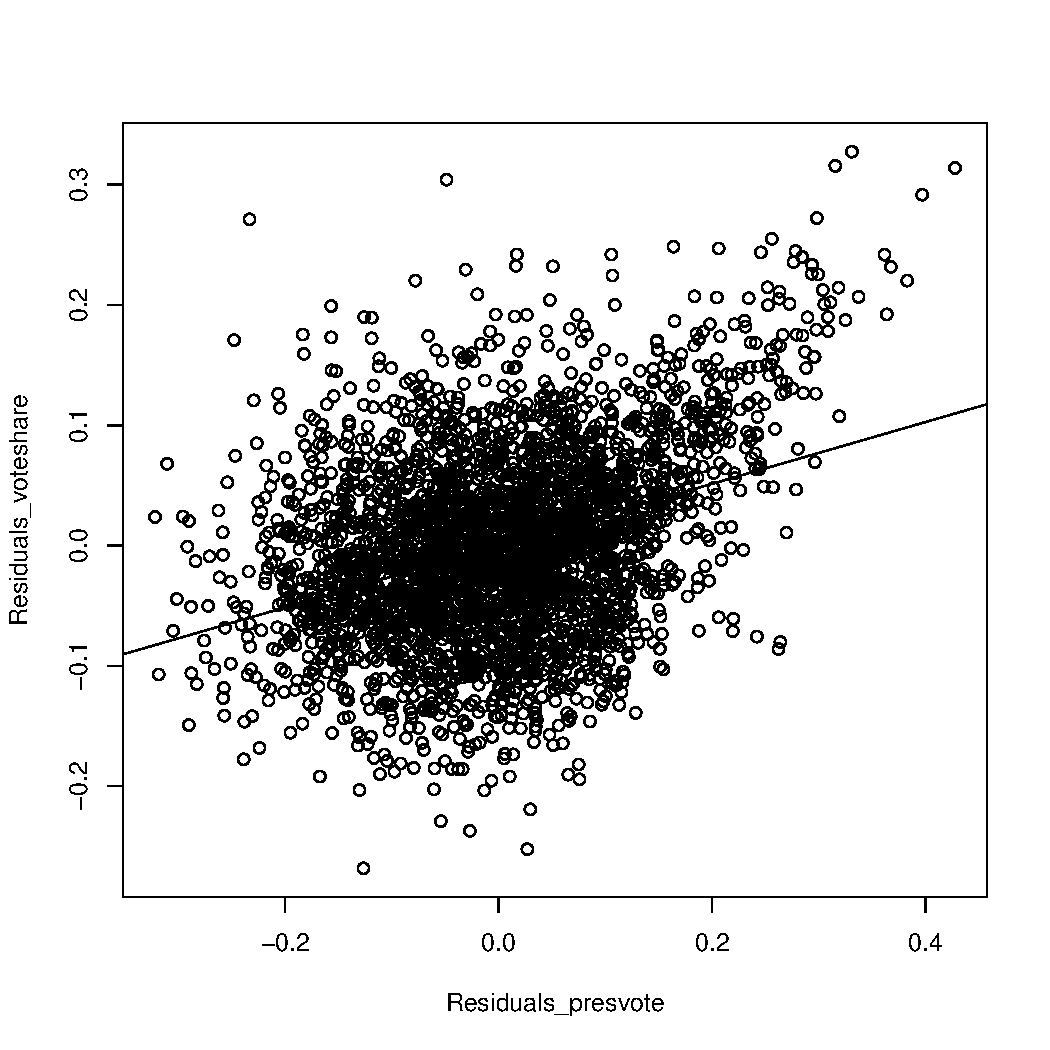
\includegraphics[width=.5\textwidth]{plotres_diffpres_diffvote.pdf}
\end{figure}
		\item Write the prediction equation.
\noindent Retrieving the coefficients from Q4.1, we get: Residuals of incumbent party voteshare = -4.860e-18 + 2.569e-01*residuals of incumbent party's presidential voteshare, or Y = -4.860e-18 + 2.569e-01X.\\
\noindent After rounding the coefficients:\\
\begin{verbatim}
> round(-4.860e-18, digits = 4)
[1] 0
> round(2.569e-01, digits = 4)
[1] 0.2569
\end{verbatim}
\noindent We get: Y = 0 + 0.2569X1 = 0.2569X1\\
	\end{enumerate}
	
	\newpage	

\section*{Question 5}
\noindent What if the incumbent's vote share is affected by both the president's popularity and the difference in spending between incumbent and challenger? 
	\begin{enumerate}
		\item Run a regression where the outcome variable is the incumbent's \texttt{voteshare} and the explanatory variables are \texttt{difflog} and \texttt{presvote}.	
\vspace{.5cm}
\lstinputlisting[language=R, firstline=123, lastline=125]{PS3_answers_LinetteLim.R}  
\vspace{.5cm}  
\noindent We get:\\
\begin{verbatim}
> summary(reg2)

Call:
lm(formula = voteshare ~ difflog + presvote, data = data)

Residuals:
     Min       1Q   Median       3Q      Max 
-0.25928 -0.04737 -0.00121  0.04618  0.33126 

Coefficients:
             Estimate Std. Error t value Pr(>|t|)    
(Intercept) 0.4486442  0.0063297   70.88   <2e-16 ***
difflog     0.0355431  0.0009455   37.59   <2e-16 ***
presvote    0.2568770  0.0117637   21.84   <2e-16 ***
---
Signif. codes:  0 ‘***’ 0.001 ‘**’ 0.01 ‘*’ 0.05 ‘.’ 0.1 ‘ ’ 1

Residual standard error: 0.07339 on 3190 degrees of freedom
Multiple R-squared:  0.4496,	Adjusted R-squared:  0.4493 
F-statistic:  1303 on 2 and 3190 DF,  p-value: < 2.2e-16
\end{verbatim}
		\item Write the prediction equation.\\
\noindent The prediction equation is Y = b0 + b1X1 + b2X2. In other words, it is: Incumbent party voteshare = 0.45 + 0.04*difference in campaign spending + 0.26*incumbent party's presidential voteshare, or Y = 0.45 + 0.04X1 + 0.26X2\\
		\item What is it in this output that is identical to the output in Question 4? Why do you think this is the case?\\
\noindent Looking at the regression output for Q5, we see that the coefficient estimate for presvote (0.2568770). This means that for a 1 unit increase in incumbent party's presidential voteshare, we have a 0.26 unit increase in incumbent pary voteshare. Comparing it with the regression output for Q4, we see that the coefficient estimate for diffpres.res (0.26) is identical to the coefficent estimate for presvote in Q5. Recall that in Q4, we regressed the residuals from voteshare ~ difflog against the residuals from presvote ~ difflog. By doing so, we are controlling for difflog (the difference in campaign spend between incumbent and challenger). In other words, this  comparison affirms the impact of presvote on voteshare as 0.26.\\
	\end{enumerate}




\end{document}
